\documentclass[tikz,border=14pt]{standalone}
\usepackage{tikz}
\usetikzlibrary{positioning, arrows.meta, calc, backgrounds}

\definecolor{ctrlFill}{RGB}{255,224,189}
\definecolor{ctrlBrd}{RGB}{204,120,30}
\definecolor{compFill}{RGB}{255,252,204}
\definecolor{compBrd}{RGB}{180,160,40}
\definecolor{locFill}{RGB}{210,235,210}
\definecolor{locBrd}{RGB}{90,150,90}
\definecolor{gloFill}{RGB}{210,225,245}
\definecolor{gloBrd}{RGB}{80,110,180}
\definecolor{gmFill}{RGB}{245,210,210}
\definecolor{gmBrd}{RGB}{180,80,80}
\definecolor{keyBg}{RGB}{245,245,245}

\tikzset{
  every node/.style={font=\ttfamily\small},
  B/.style={draw, rounded corners=1pt, inner sep=4pt, align=center, minimum height=0.65cm},
  CTRL/.style={B, fill=ctrlFill, draw=ctrlBrd},
  COMP/.style={B, fill=compFill, draw=compBrd},
  LOC/.style={B,  fill=locFill,  draw=locBrd},
  GLO/.style={B,  fill=gloFill,  draw=gloBrd},
  GM/.style={B,   fill=gmFill,   draw=gmBrd},
  AR/.style={-{Stealth[length=5pt]}, thick, black, shorten >=8pt, shorten <=8pt},
}

\newcommand{\vflow}[2]{\draw[AR] (#1.south) -- (#2.north);}

\begin{document}
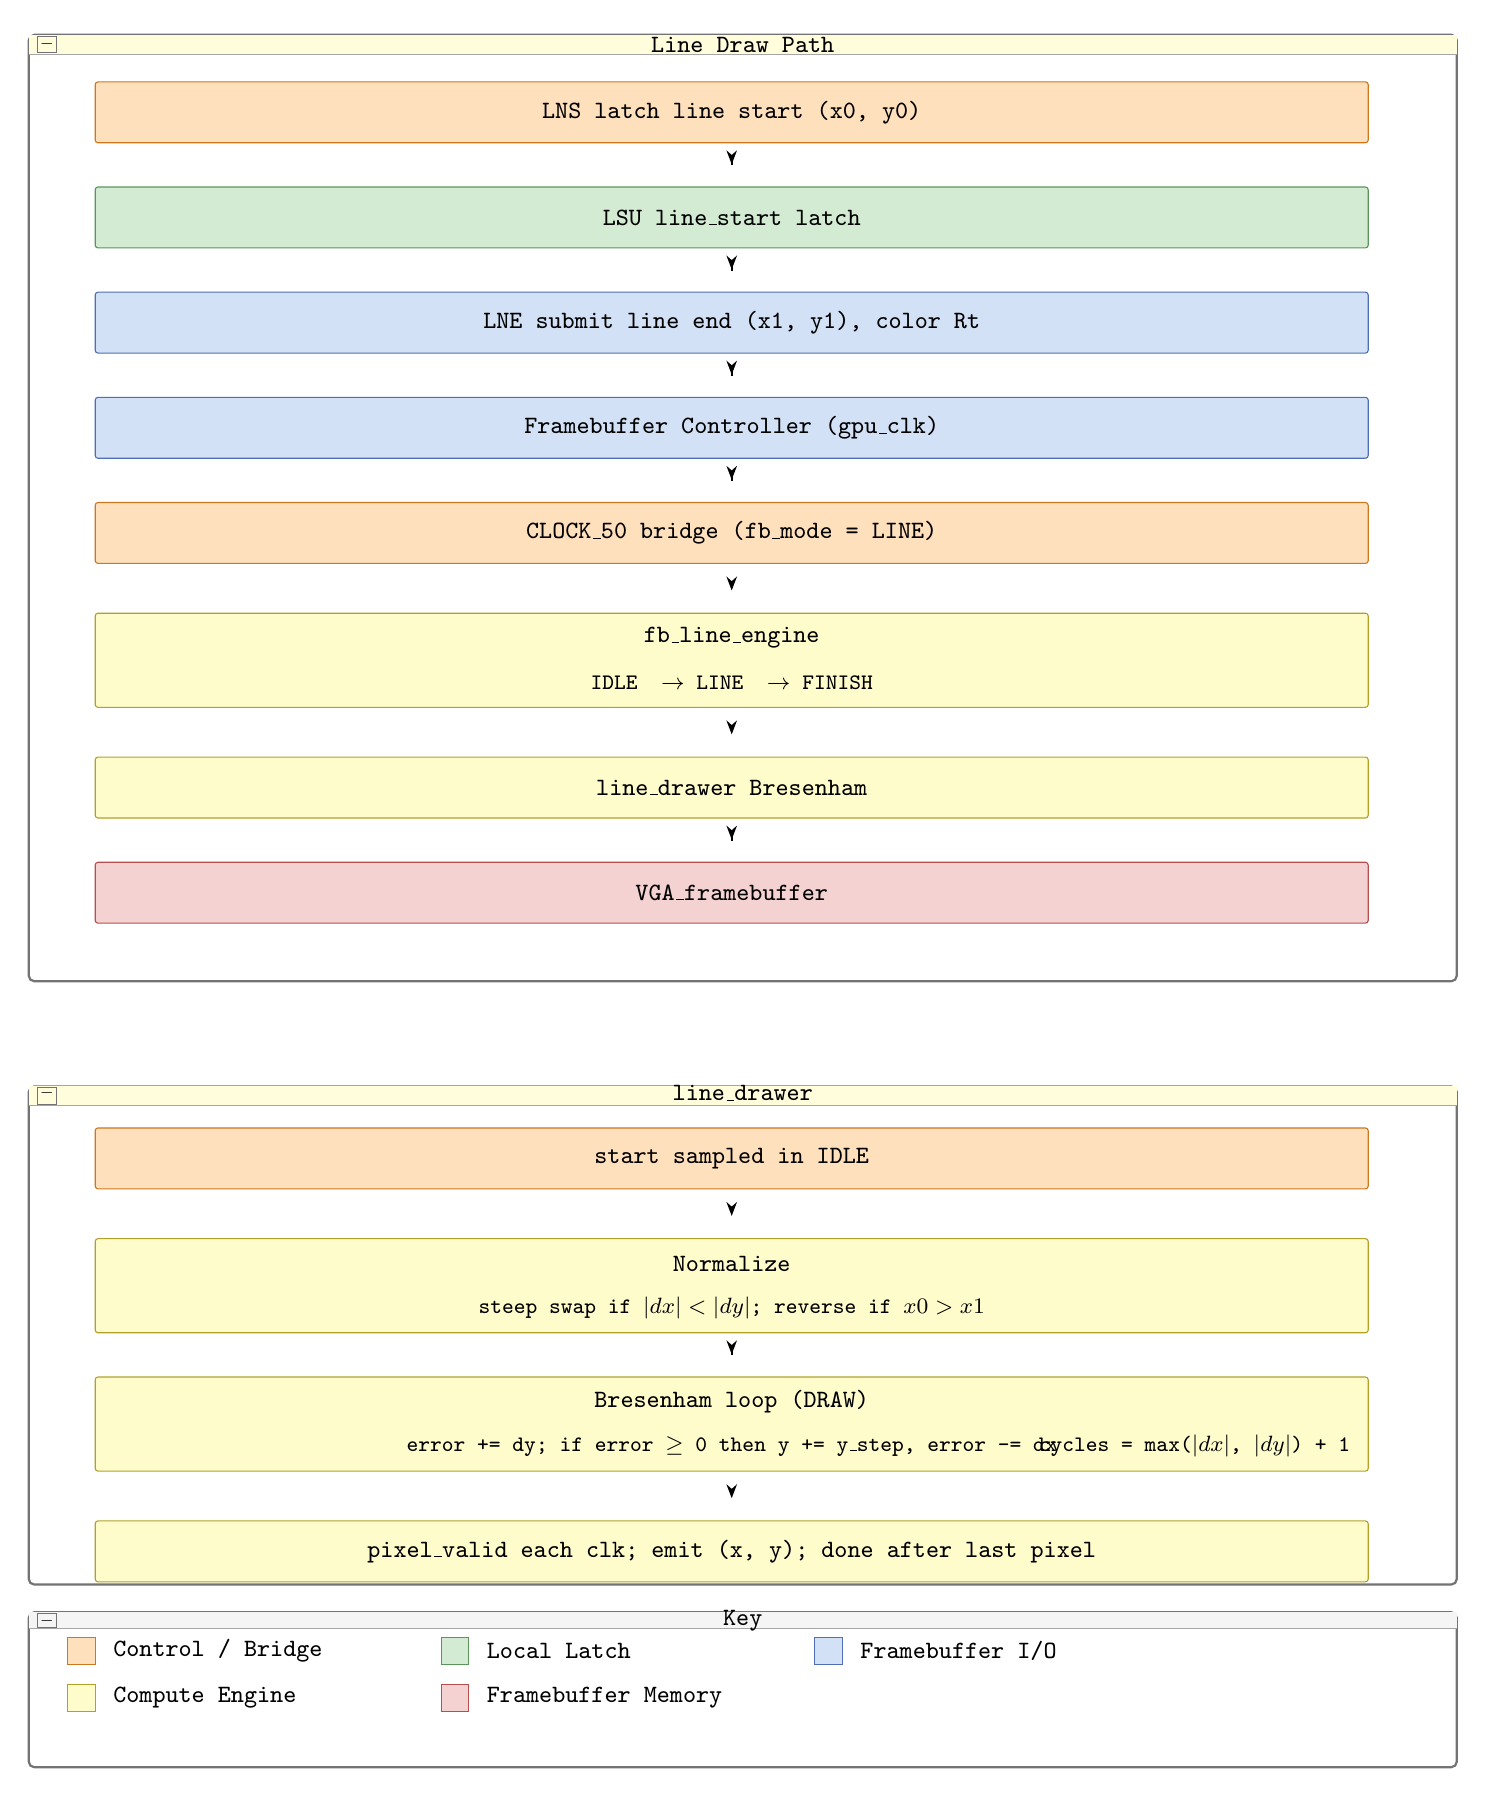
\begin{tikzpicture}[x=1pt, y=1pt, yscale=-1]

\def\W{460pt}
\def\cx{260}

%% ═══════════════════════════════════════════════════════════════════════════
%%  Panel A — end-to-end line draw path (GPU -> framebuffer)
%% ═══════════════════════════════════════════════════════════════════════════

\node[CTRL, minimum width=\W, minimum height=22pt] (LNS) at (\cx,16)
  {\textbf{LNS} latch line start (x0, y0)};
\node[LOC, minimum width=\W, minimum height=22pt] (LAT) at (\cx,54)
  {LSU line\_start latch};
\node[GLO, minimum width=\W, minimum height=22pt] (LNE) at (\cx,92)
  {\textbf{LNE} submit line end (x1, y1), color Rt};
\node[GLO, minimum width=\W, minimum height=22pt] (FBC) at (\cx,130)
  {Framebuffer Controller (gpu\_clk)};
\node[CTRL, minimum width=\W, minimum height=22pt] (BRG) at (\cx,168)
  {CLOCK\_50 bridge (fb\_mode = LINE)};
\node[COMP, minimum width=\W, minimum height=34pt] (ENG) at (\cx,214) {};
\node[font=\ttfamily\small\bfseries] at (\cx,206) {fb\_line\_engine};
\node[font=\ttfamily\footnotesize] at (\cx,222)
  {IDLE \enspace$\rightarrow$\enspace LINE \enspace$\rightarrow$\enspace FINISH};
\node[COMP, minimum width=\W, minimum height=22pt] (LD) at (\cx,260)
  {\textbf{line\_drawer} Bresenham};
\node[GM, minimum width=\W, minimum height=22pt] (FB) at (\cx,298)
  {VGA\_framebuffer};

\vflow{LNS}{LAT}
\vflow{LAT}{LNE}
\vflow{LNE}{FBC}
\vflow{FBC}{BRG}
\vflow{BRG}{ENG}
\vflow{ENG}{LD}
\vflow{LD}{FB}

\begin{scope}[on background layer]
  \draw[black!55,thick,rounded corners=2pt] (6,-12) rectangle (522,330);
  \fill[compFill!70] (6,-12) rectangle (522,-5);
  \draw[black!35] (6,-5)--(522,-5);
\end{scope}
\node[font=\ttfamily\small\bfseries] at (264,-8.5) {Line Draw Path};
\draw[black!55] (9,-11.5) rectangle (16,-5.5);
\node[font=\ttfamily\tiny] at (12.5,-8.5) {$-$};

%% ═══════════════════════════════════════════════════════════════════════════
%%  Panel B — line_drawer internals
%% ═══════════════════════════════════════════════════════════════════════════

\def\yTop{368}
\def\yB{394}
\node[CTRL, minimum width=\W, minimum height=22pt] (S0) at (\cx,\yB)
  {start sampled in IDLE};
\node[COMP, minimum width=\W, minimum height=34pt] (NORM) at (\cx,\yB+46) {};
\node[font=\ttfamily\small\bfseries] at (\cx,\yB+38) {Normalize};
\node[font=\ttfamily\footnotesize] at (\cx,\yB+54)
  {steep swap if $|dx|<|dy|$; reverse if $x0>x1$};
\node[COMP, minimum width=\W, minimum height=34pt] (BRES) at (\cx,\yB+96) {};
\node[font=\ttfamily\small\bfseries] at (\cx,\yB+88) {Bresenham loop (DRAW)};
\node[font=\ttfamily\footnotesize] at (\cx,\yB+104)
  {error += dy; if error $\geq$ 0 then y += y\_step, error -= dx};
\node[COMP, minimum width=\W, minimum height=22pt] (OUT) at (\cx,\yB+142)
  {pixel\_valid each clk; emit (x, y); done after last pixel};

\vflow{S0}{NORM}
\vflow{NORM}{BRES}
\vflow{BRES}{OUT}

\node[font=\ttfamily\footnotesize, anchor=east] at (487,\yB+104)
  {cycles = max($|dx|$, $|dy|$) + 1};

\def\yBot{548}
\begin{scope}[on background layer]
  \draw[black!55,thick,rounded corners=2pt] (6,\yTop) rectangle (522,\yBot);
  \fill[compFill!70] (6,\yTop) rectangle (522,\yTop+7);
  \draw[black!35] (6,\yTop+7)--(522,\yTop+7);
\end{scope}
\node[font=\ttfamily\small\bfseries] at (264,\yTop+2.5) {line\_drawer};
\draw[black!55] (9,\yTop+0.5) rectangle (16,\yTop+6.5);
\node[font=\ttfamily\tiny] at (12.5,\yTop+2.5) {$-$};

%% Key
\def\yKeyTop{558}
\def\yKeyBot{614}
\begin{scope}[on background layer]
  \draw[black!55,thick,rounded corners=2pt] (6,\yKeyTop) rectangle (522,\yKeyBot);
  \fill[keyBg] (6,\yKeyTop) rectangle (522,\yKeyTop+6);
  \draw[black!35] (6,\yKeyTop+6)--(522,\yKeyTop+6);
\end{scope}
\node[font=\ttfamily\small] at (264,\yKeyTop+3) {Key};
\draw[black!55] (9,\yKeyTop+0.5) rectangle (16,\yKeyTop+5.5);
\node[font=\ttfamily\tiny] at (12.5,\yKeyTop+3) {$-$};

\fill[ctrlFill](20,\yKeyTop+9) rectangle(30,\yKeyTop+19); \draw[ctrlBrd](20,\yKeyTop+9) rectangle(30,\yKeyTop+19);
\node[anchor=west,font=\ttfamily\small] at (33,\yKeyTop+14) {Control / Bridge};
\fill[locFill] (155,\yKeyTop+9) rectangle(165,\yKeyTop+19); \draw[locBrd](155,\yKeyTop+9) rectangle(165,\yKeyTop+19);
\node[anchor=west,font=\ttfamily\small] at (168,\yKeyTop+14) {Local Latch};
\fill[gloFill] (290,\yKeyTop+9) rectangle(300,\yKeyTop+19); \draw[gloBrd](290,\yKeyTop+9) rectangle(300,\yKeyTop+19);
\node[anchor=west,font=\ttfamily\small] at (303,\yKeyTop+14) {Framebuffer I/O};
\fill[compFill](20,\yKeyTop+26) rectangle(30,\yKeyTop+36); \draw[compBrd](20,\yKeyTop+26) rectangle(30,\yKeyTop+36);
\node[anchor=west,font=\ttfamily\small] at (33,\yKeyTop+31) {Compute Engine};
\fill[gmFill]  (155,\yKeyTop+26) rectangle(165,\yKeyTop+36); \draw[gmBrd](155,\yKeyTop+26) rectangle(165,\yKeyTop+36);
\node[anchor=west,font=\ttfamily\small] at (168,\yKeyTop+31) {Framebuffer Memory};

\end{tikzpicture}
\end{document}
